\subsection{API Specification}

Socket.io uses message-passing mechanism to communicate and send/receive data. Different types of messages are identified via its message name; therefore we build a set of message types that is used as APIs that help the server and clients interact between each other.

Here shows the complete list of APIs:

\begin{center}

\begin{tabular}{| l | l | p{7.5cm} |}

\hline
API name & Direction & Description \\
\hline
MAPSTART & Server to client & The server sends split data, mapper, emitter and reducer functions to the client and tells the client to start mapper task. \newline
Note that the mapper, emitter and reducer in the message body are just plain strings, but can be translated back to functions. \newline
The emitter will be executed inside the mapper function in order to summarize the outputs by the mapper. \\
\hline
MAPDATA & Client to Server & The client sends the mapper output to the server. \newline
Upon receiving MAPDATA, the server will use handshaking to notify the client, which will then emits the MAPEND message. \\
\hline
MAPEND & Client to Server & The client tells the server that the mapper phase has completed. \\
\hline
REDUCE & Server to Client & The server sends the message with a key-value pair, and tells the client to execute reducer task by using the key-value pair as the input. \\
\hline
MAP\_ALL\_END & Server to Client & The server tells all clients that \newline
(1) all mapper tasks are done and \newline
(2) all REDUCE messages has been sent and \emph{received} by all clients. \newline
Thus the clients can therefore upload the output data of reducers. \newline
This message will be broadcasted while satisfying two conditions: \newline
(1) the server receives all MAPEND messages. \newline
(2) the server knows that all REDUCE messages has been received. \\
\hline
REDUCEDATA & Client to Server & The client uploads the output data of reducer to the server. \newline
The message will be sent while the client receives MAP\_ALL\_END message. If there are still some reducers running, the message will be sent right after all reducers are terminated; otherwise it will be sent directly after ceceiving MAP\_ALL\_END. \newline
Upon receiving the message, the server uses handshaking to notify the client, which will then emits the REDUCEEND message. \\
\hline
REDUCEEND & Client to Server & The client tells the server that the reduce phase has completed. \\
\hline
COMPLETE & Server to Client & The server tells all clients that the whole program has completed. A brief summary is sent in the message body. \\
\hline

\end{tabular}

\end{center}

After explained those APIs in detail, we illustrate the overview of the execution flow, which is complicated due to the communications between the server and the clients. The sequence diagram below describes the execution in detail.

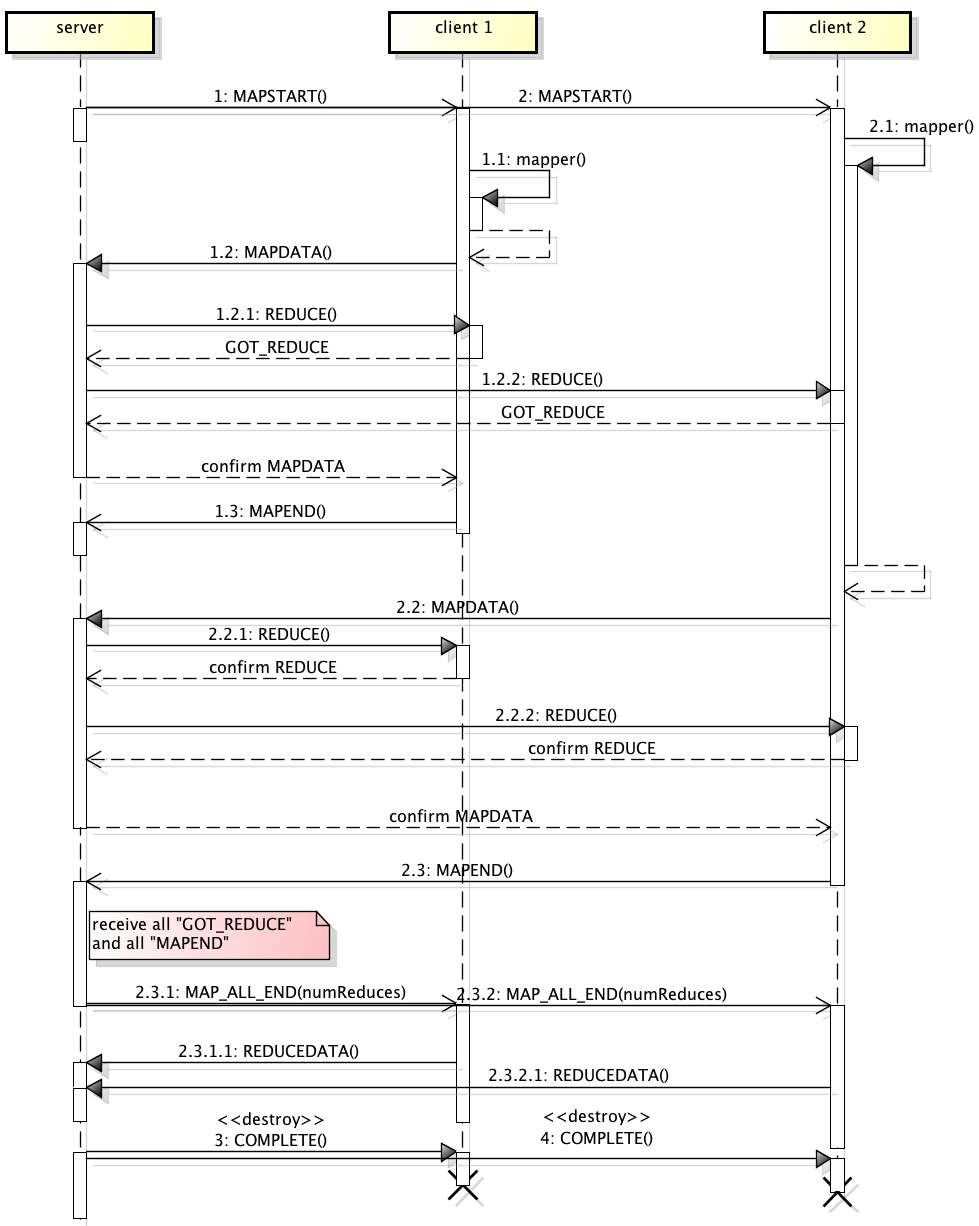
\includegraphics[width=12.5cm, keepaspectratio=true]{JSMP.png}
